\section{\ours：通过 RL 为 VLM 启动工具集成推理能力}
\label{sec:training}

\subsection{两阶段训练框架}
基于 \env{}，我们构建了一个两阶段训练框架。第一阶段使用行为克隆（BC）启动一个可交互智能体，为其注入指令跟随和基础工具使用能力；第二阶段则使用多轮在线 RL 进一步优化，使模型获得更深层推理能力以及由推理驱动的工具编排能力。

\noindent \textbf{阶段 I：模仿学习预热。}
我们首先在合成专家轨迹上执行 BC，这些轨迹\emph{显式地}交错包含思考与动作。具体流程包括：(i) \textit{候选生成与过滤。} 我们先用闭源模型 \texttt{GPT‑5} 生成带工具执行的候选轨迹，只保留最终答案与真值完全一致的样本；(ii) \textit{推理轨迹增密。} 为了加强对推理过程的监督，我们用开源专家 \texttt{Qwen3‑VL‑235B‑A22B‑Thinking} 生成更长、更丰富的推理轨迹，替换原本较简洁的 rationale。记最终数据集为 $\mathcal{D}$，其中每个样本是 $(x,\tau)$，$\tau{=}(g_1,a_1,\ldots,g_T,\hat{y})$。BC 目标就是最大化这些交错 thought–action 序列的似然：
\begin{equation*}
    \begin{aligned}
        &\mathcal{L}_{\text{BC}}(\theta)=\mathbb{E}_{(x,\tau)\sim\mathcal{D}}[\log\pi_\theta(\tau|x)]\\
        &=\mathbb{E}\left[\sum_{t=0}^{T-1}\log\pi_\theta(a_t|x,c_{t-1},g_t)+\sum_{t=0}^{T}\log\pi_\theta(g_t|x,c_{t-1})\right].
    \end{aligned}
\end{equation*}
这一合成语料覆盖了丰富的工具组合（图~\ref{fig:sft-tool-distribution}），因此为工具语法和工具选择提供了稳健先验。

\noindent \textbf{阶段 II：在线 RL。}
在 SFT 之后，我们在可执行环境中对智能体进行多轮 rollout 训练。每一步先输出推理段，再输出函数调用；\env{} 执行该调用，并把结构化反馈追加到上下文中，供后续继续推理。我们采用 Group Relative Policy Optimization（GRPO）~\cite{shao2024deepseekmath} 进行策略改进，对 $G$ 条 rollout 使用组归一化优势：
\begin{equation*}
    \begin{aligned}
        \mathcal{L}_{\text{GRPO}}(\theta)&=\frac{1}{G}\sum_{i=1}^G\frac{1}{|\tau_i|}\sum_{k=1}^{|\tau_i|}\min[r_{i,k}(\theta)\cdot\hat{A}_{i,k},\\
        &\quad\text{clip}(r_{i,k}(\theta),1-\epsilon,1+\epsilon)\cdot\hat{A}_{i,k}],
    \end{aligned}
\end{equation*}
其中 $r_{i,k}(\theta)$ 表示第 $k$ 个 token 的重要性比例：
\begin{equation*}
    \begin{aligned}
        r_{i,k}(\theta)&=\frac{\pi_\theta(\tau_{i,k}|\tau_{i,<k})}{\pi_{\text{old}}(\tau_{i,k}|\tau_{i,<k})},
    \end{aligned}
\end{equation*}
而 $\hat{A}_{i,k}$ 则是基于 rollout 级奖励 $R(\tau_i)$ 计算得到的归一化优势：
\begin{equation*}
    \begin{aligned}
        \quad \hat{A}_{i,k}&=\frac{R(\tau_i)-\text{mean}(\{R(\tau_1),\cdots,R(\tau_G)\}}{\text{std}(\{R(\tau_1),\cdots,R(\tau_G)\})}.
    \end{aligned}
\end{equation*}

我们采用多轮交互协议 $U=(u_0,u_1,\cdots,u_{T})$ 进行训练，并围绕这一协议设计奖励 $R$。该协议要求每个 turn 都遵守显式的 \textit{think}$\rightarrow$\textit{tool\_call} 循环，最后以 \textit{think}$\rightarrow$\textit{answer} 结束：

\noindent~$\bullet$ \textbf{Turn ($<T$)（工具调用）：}
\begin{equation*}
    \begin{aligned} u_{i<T}=\text{<think>}\cdots\text{</think>}\text{<tool\_call>}\cdots\text{</tool\_call>}.
    \end{aligned}
\end{equation*}

\noindent~$\bullet$ \textbf{Turn $T$（最终答案）：}
\begin{equation*}
    \begin{aligned}
u_T=\text{<think>}\cdots\text{</think>}\text{<answer>}\cdots\text{</answer>}.
    \end{aligned}
\end{equation*}

\noindent\textbf{重复惩罚。}
我们首先应用高优先级重复检测器 $R_{\text{rep}}(U)\!\in\!\{-3.0,-2.0,-1.5,0\}$，检查连续 token、词组或字符重复，并按严重程度给予负奖励（极端、严重、中等、无）。这一项具有最高优先级。

\noindent\textbf{格式奖励。}
在\emph{无重复}条件下，即 $R_{\text{rep}}(U){=}0$，我们验证每一轮输出是否结构良好，例如标签是否正确、顺序是否正确、闭合是否非嵌套。形式化地，
\begin{equation*}
    \begin{aligned}
        R_{\text{format}}(U)=(\mathbb{I}\{\text{all $u_i$ conforms the format}\}-0.5)\times2.
    \end{aligned}
\end{equation*}

\noindent\textbf{正确性奖励。}
我们从 \texttt{<answer>}…\texttt{</answer>} 中提取最终预测 $\hat{y}$，并以规则方式校验其正确性。为保持信号低噪声并与格式一致性对齐，我们只对无重复且格式正确的输出给予正确性奖励：
\begin{equation*}
    \begin{aligned}
        R_{\text{correct}}(U)=\mathbb{I}\{\hat{y}=y\}.
    \end{aligned}
\end{equation*}

\noindent\textbf{最终奖励。}
轨迹级奖励由三部分相加得到：
\begin{equation*}
    \begin{aligned}
        R(U)=R_{\text{rep}}(U)+R_{\text{format}}(U)+R_{\text{correct}}(U).
    \end{aligned}
\end{equation*}
这种稀疏且格式敏感的奖励设计，只对“无重复、结构正确且答案正确”的生成给予正反馈，从而鼓励策略学习我们期望的 \textit{think}$\rightarrow$\textit{tool\_call}$\rightarrow$\textit{answer} 协议，而不是依赖中间启发式捷径。

\begin{figure}
    \centering
    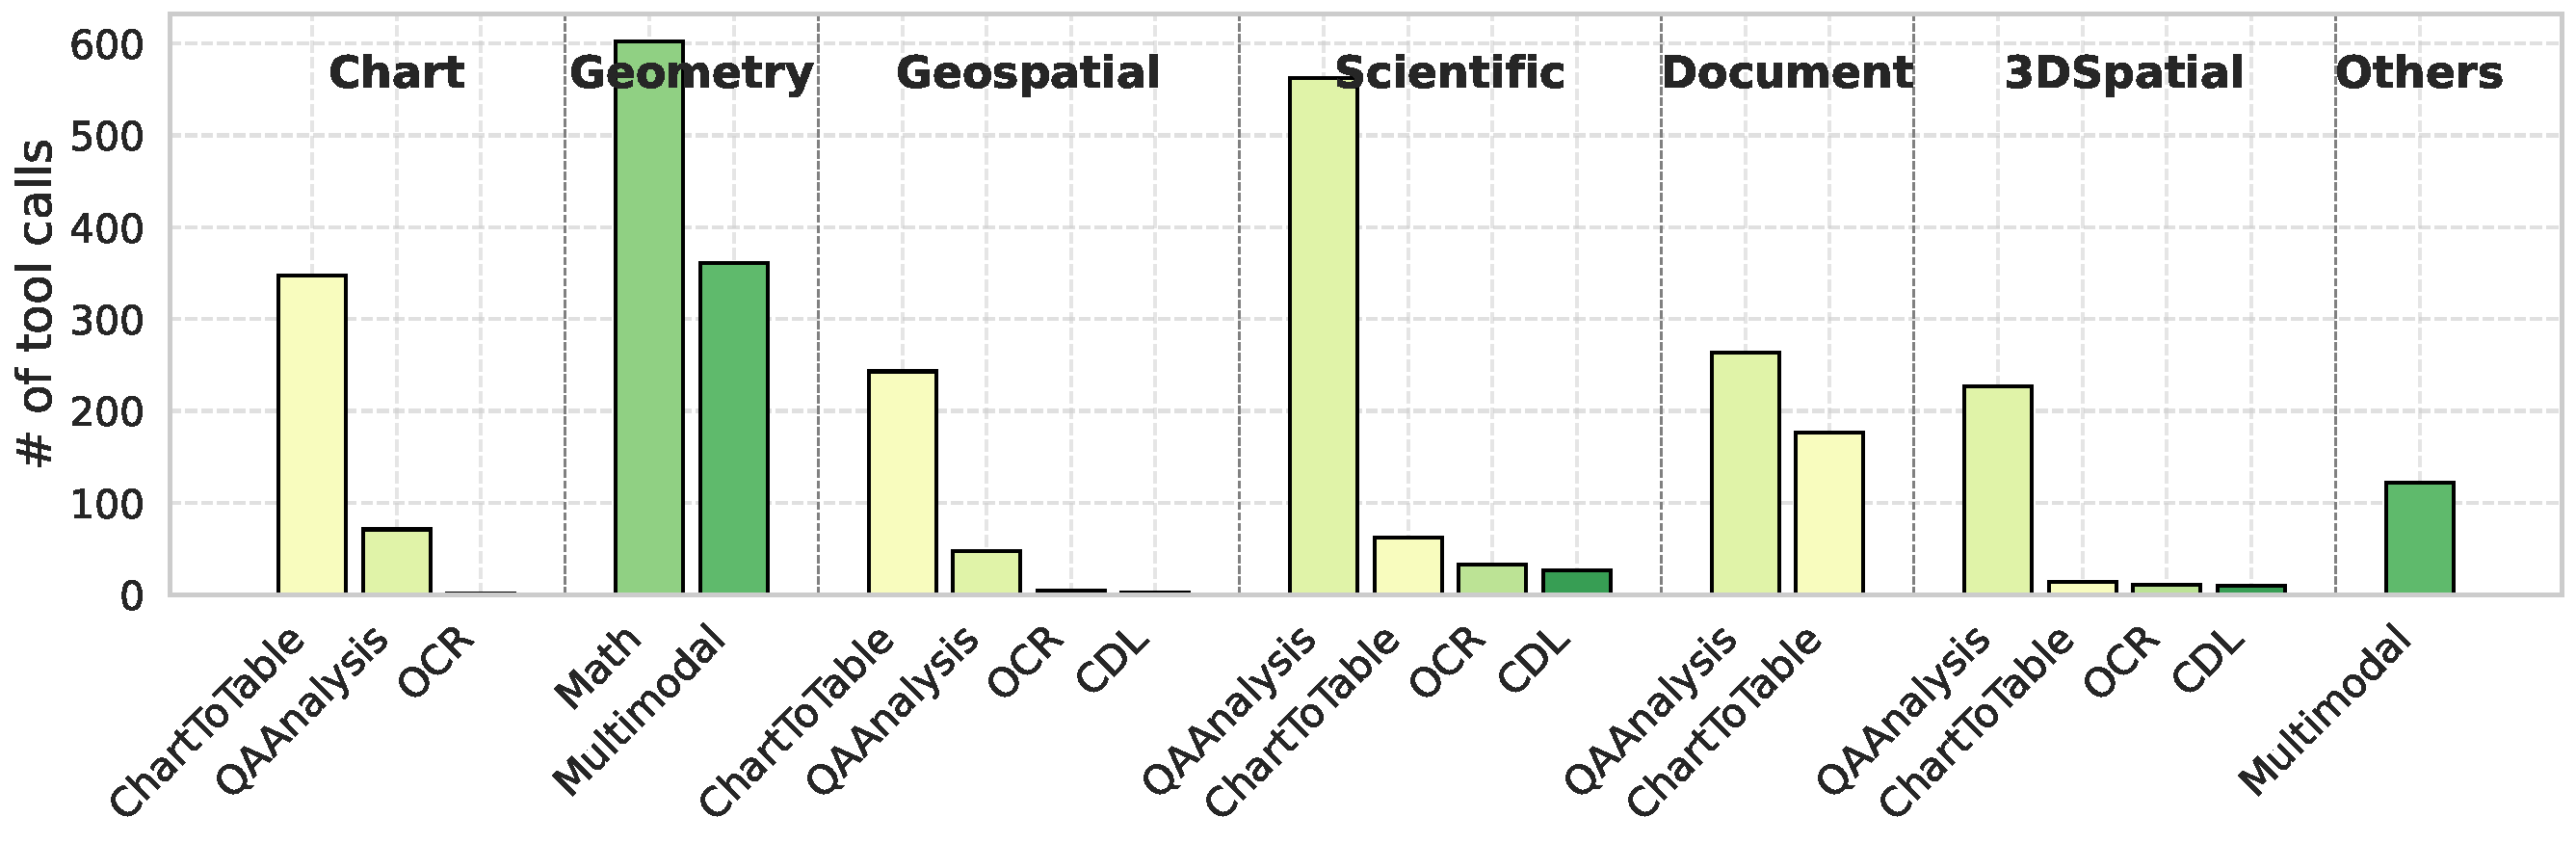
\includegraphics[width=\linewidth]{figure/tool-distribution.pdf}
    \caption{SFT 数据中不同任务的主要工具调用分布。}
    \label{fig:sft-tool-distribution}
\end{figure}
